\section{Background and Motivation}
    \begin{frame}{Background and Motivation}
        \vspace{0.5mm}
        {\bf BACKGROUND}: Salomon has run beam simulations in {\tt GENE}, using 3 (4) species:
        \vspace{0.5mm}
        {\footnotesize \begin{center}\begin{tabular}{ c || c | c | c }
            Species  &  Particle  &  Density  &  Distribution  \\
            \hline\hline
            Electrons  &  Electron  &  High  &  Maxwellian$\left\{\begin{aligned}  {\sf Velocity}  &=  \bfzero 
    \\  {\sf Temperature}  &=  {\sf Low}  \end{aligned}\right.$  \\
            \hline
            Ions  &  Proton  &  High  &  Maxwellian$\left\{\begin{aligned}  {\sf Velocity}  &=  \bfzero 
    \\  {\sf Temperature}  &=  {\sf Low}  \end{aligned}\right.$  \\
            \hline
            Beam  &  Proton  &  Low  &  Maxwellian$\left\{\begin{aligned}  {\sf Velocity}  &=  \bfzero
    \\  {\sf Temperature}  &=  {\sf High}  \end{aligned}\right.$
        \end{tabular}\end{center}}  \pause
        
        \begin{alertblock}{\bf CRITICISM}
            \begin{itemize}
                \item  Poorly represented beam distribution function!

                \item  Can we improve this?
            \end{itemize}
        \end{alertblock}
    \end{frame}
    
    \begin{frame}{Background and Motivation}
        \vspace{0.5mm}
        {\bf BACKGROUND}: Salomon has run beam simulations in {\tt GENE}, using 3 (4) species:
        \vspace{0.5mm}
        {\footnotesize \begin{center}\begin{tabular}{ c || c | c | c }
            Species  &  Particle  &  Density  &  Distribution  \\
            \hline\hline
            Electrons  &  Electron  &  High  &  Maxwellian$\left\{\begin{aligned}  {\sf Velocity}  &=  \bfzero 
    \\  {\sf Temperature}  &=  {\sf Low}  \end{aligned}\right.$  \\
            \hline
            Ions  &  Proton  &  High  &  Maxwellian$\left\{\begin{aligned}  {\sf Velocity}  &=  \bfzero 
    \\  {\sf Temperature}  &=  {\sf Low}  \end{aligned}\right.$  \\
            \hline
            Beam  &  Proton  &  Low  &  {\color{red!90} Maxwellian$\left\{\begin{aligned}  {\sf Velocity}  &=  \bfzero
    \\  {\sf Temperature}  &=  {\sf High}  \end{aligned}\right.$}
        \end{tabular}\end{center}}
        
        \begin{alertblock}{\bf CRITICISM}
            \begin{itemize}
                \item  Poorly represented beam distribution function!

                \item  Can we improve this?
            \end{itemize}
        \end{alertblock}
    \end{frame}
    
    \begin{frame}{Background and Motivation}
        \vspace{0.5mm}
        {\bf BACKGROUND}: Salomon has run beam simulations in {\tt GENE}, using 3 (4) species:
        \vspace{0.5mm}
        {\footnotesize \begin{center}\begin{tabular}{ c || c | c | c }
            Species  &  Particle  &  Density  &  Distribution  \\
            \hline\hline
            Electrons  &  Electron  &  High  &  Maxwellian$\left\{\begin{aligned}  {\sf Velocity}  &=  \bfzero 
    \\  {\sf Temperature}  &=  {\sf Low}  \end{aligned}\right.$  \\
            \hline
            Ions  &  Proton  &  High  &  Maxwellian$\left\{\begin{aligned}  {\sf Velocity}  &=  \bfzero 
    \\  {\sf Temperature}  &=  {\sf Low}  \end{aligned}\right.$  \\
            \hline
            Beam  &  Proton  &  Low  &  {\color{red!90} Maxwellian$\left\{\begin{aligned}  {\sf Velocity}  &=  {\sf Non-}\bfzero
    \\  {\sf Temperature}  &=  {\sf High}  \end{aligned}\right.$}
        \end{tabular}\end{center}}
        
        \begin{alertblock}{\bf CRITICISM}
            \begin{itemize}
                \item  Poorly represented beam distribution function!

                \item  Can we improve this?
            \end{itemize}
        \end{alertblock}
    \end{frame}
    
    \begin{frame}{Background and Motivation}    
        \begin{figure}
            \centering
            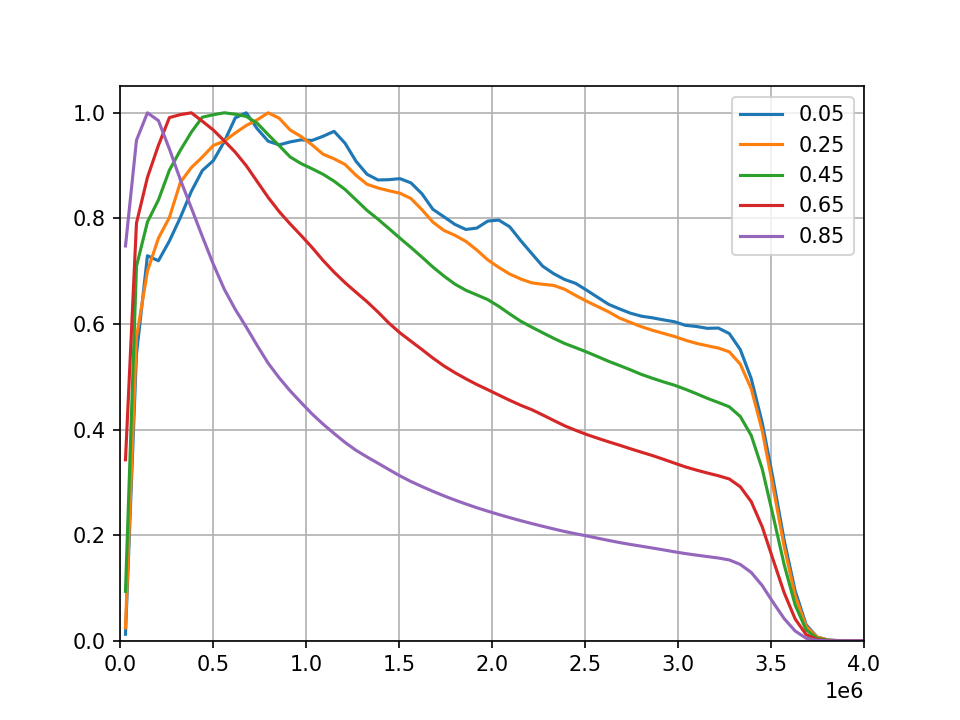
\includegraphics[width = 0.65\textwidth]{1 - background and motivation/images/Experimental Damped Distributions.png}
            \caption{Energy density profiles (on different flux tubes) showing the damping of (alpha) particles over a certain threshold energy(/velocity)}
        \end{figure}
    \end{frame}
    
    \begin{frame}{Background and Motivation}
        \vspace{0.5mm}
        {\bf BACKGROUND}: Salomon has run beam simulations in {\tt GENE}, using 3 (4) species:
        \vspace{0.5mm}
        {\footnotesize \begin{center}\begin{tabular}{ c || c | c | c }
            Species  &  Particle  &  Density  &  Distribution  \\
            \hline\hline
            Electrons  &  Electron  &  High  &  Maxwellian$\left\{\begin{aligned}  {\sf Velocity}  &=  \bfzero 
    \\  {\sf Temperature}  &=  {\sf Low}  \end{aligned}\right.$  \\
            \hline
            Ions  &  Proton  &  High  &  Maxwellian$\left\{\begin{aligned}  {\sf Velocity}  &=  \bfzero 
    \\  {\sf Temperature}  &=  {\sf Low}  \end{aligned}\right.$  \\
            \hline
            Beam  &  Proton  &  Low  &  {\color{red!90} $\begin{aligned} 
     {\sf Damped}  \\  {\sf Maxwellian}  \end{aligned}\left\{\begin{aligned}  {\sf Velocity}  &=  {\sf Non-}\bfzero 
        \\  {\sf Temperature}  &=  {\sf High}  \\  \begin{aligned} 
     {\sf Damping}  \\  {\sf speed}  \end{aligned}  &=  v_{A}  \end{aligned}\right.$}
        \end{tabular}\end{center}}
    \end{frame}

    \begin{frame}{Background and Motivation}
        \begin{alertblock}{\bf PROBLEM}
            {\tt GENE} supports:
            \begin{itemize}
                \item[\bftick]  \emph{Maxwellian} backgrounds
                \item[\ast]  \emph{Shifted Maxwellian} backgrounds
                \item[\bfcross]  \emph{Fully non-Maxwellian} backgrounds (i.e. here damped distributions)
            \end{itemize}
        \end{alertblock}  \pause
        
        \begin{block}{\bf PROJECT}
            \begin{itemize}
                \item  \emph{Fix} generic background distributions support
                \item  \emph{Add} damped Maxwellians
            \end{itemize}
        \end{block}
    \end{frame}